\section{Labor 1}
In \cite[S. 12]{Mazzetti1996} der Laborübung sollen erste Erfahrungen mit der Vivado IDE und dem Xilinx SDK gemacht werden. Zunächst werden in der Vivado IDE die Verbindung des Prozessors zur Peripherie hergestellt, um anschließend mit dem SDK ein Programm schreiben zu können, was es erlaubt LEDs auf dem Zedboard blinken zu lassen.

Für diese Laborübung waren folgende Fragen als Vorbereitung zu bearbeiten:

\faq{Hat der ARM Prozessor Memory Mapped oder Isolated IO?}
    {Bei Memory Mapped werden die Register der Peripheriegeräte innerhalb des gewöhnlichen Adressraumes abgebildet und als solche angesteuert. Beim Isolated IO verwendet man hingegen einen isolierten Adressraum. Bei einem ARM Prozessor wird Memory Mapped verwendet. Das kann zum Beispiel im Dokument UG585 in der Tabelle 4-1 erkannt werden. Dort werden alle Adressen dargestellt, die sich im PS befinden.}

\subsection{Aufgabe 1}

In der ersten Aufgabe haben wir ein Block Design in der Vivado IDE erstellt. Hier gibt es eine Abweichung zur Aufgabenstellung. Wir verwenden in all unseren Laboren das Zybo-Board von Digilent, welches nur 4 LEDs besitzt. Aus Diesem Grund sind an dem AXI-GPIO0-Block nur vier LEDs angeschlossen. Im Bild \ref{Labor1_Aufgabe1_Bild1} ist das komplette Block Design dargestellt. Die Konfiguration des FPGAs ermöglicht es die LEDs über die Programmbale Logic (PL) und das Processing System (PS) anzusprechen. Dafür werden 435 LUTs, 60 LUTRAMs, 613 Flip Flops, ein BUFG und vier Inputs/Outputs verwendet.

\begin{figure}[hbt]
	\centering
	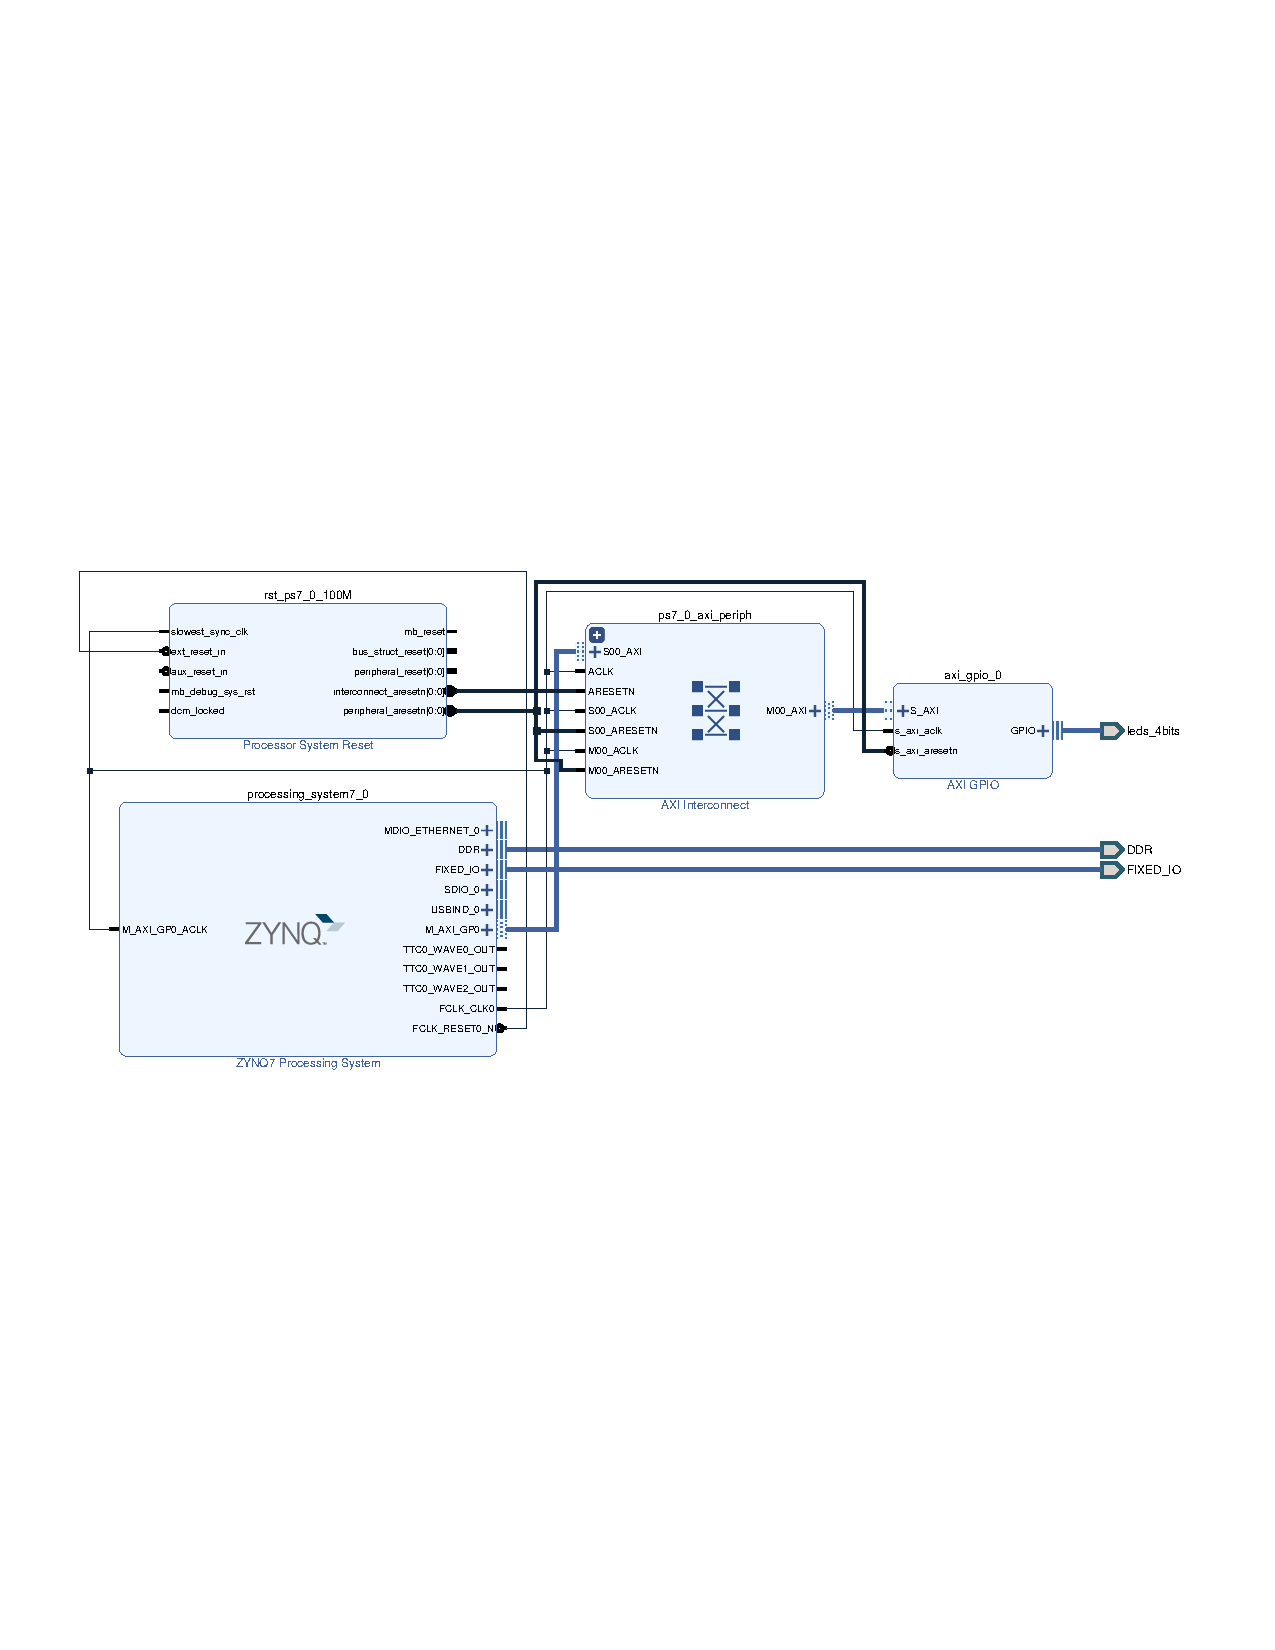
\includegraphics[trim = 10mm 100mm 10mm 100mm, width=0.9\linewidth]{./Bilder/Labor1_Aufgabe1_Bild1}
	\caption{LED Ansteuerung über AXI GPIO}
	\label{Labor1_Aufgabe1_Bild1}
\end{figure}

\subsection{Aufgabe 2}
In der Aufgabe 2 wird ein C-Programm geschrieben, um die LEDs über das PS zu steuern. Der Quellcode ist in der Aufgabenstellung gegeben und wurde nicht modifiziert.

In dem vorgegebenen Programm werden zuerst die GPIO initialisiert und danach geht das Programm in eine Endlosschleife. In der Schleife werden die LEDs in einem bestimmten Muster eingeschaltet und anschließend eine gewisse Zeit gewartet, bevor die Schleife mit dem invertierten Muster von vorne beginnt.

\faq{Wie funktioniert die Funktion XGpio\_DiscreteWrite}
    {Die hier zu beschreibende Funktion soll in ein Register schreiben, um GPIOs zu setzten. Zuerst wird der übergebene Pointer mit dem Typ XGpio überprüft, ob er gültig ist. Ist der Übergabeparameter kein Null-Pointer wird getestet, ob der GPIO-Port bereit ist und ein Kanal angegeben wurde. Ist alles korrekt wird der Pointer weiter an die Funktion XGpio\_WriteReg gegeben.}

\faq{Woran / Wo sieht man die Antwort von der Vorbereitung im Code?}
    {Über die Datei xil\_io.h kann direkt in einen Speicher geschrieben werden. Die Zuweisungen der Registeradressen sind in xparameters.h zu finden.}
    
\subsection{Aufgabe 3}
In der dritten Aufgabe sollen nicht nur die LEDs über GPIO , sondern auch die Schalter bzw. Knöpfe angesteuert werden. In Abbildung \ref{Labor1_Aufgabe3_Bild1} ist ein weiterer GPIO-Block mit dem Namen \textit{axi\_gpio\_0} hinzugekommen.

In Quellcode \ref{Labor1_Aufgabe3_Code1} werden erst die GPIOs konfiguriert und danach geht das Programm in eine Endlosschleife. In der Endlosschleife werden die Schalter ausgelesen und der ausgelesen Wert auf die LEDs angewendet. Am Ende folgt eine Pause, erst danach geht die Schleife von vorne los.

\begin{figure}[hbt]
	\centering
	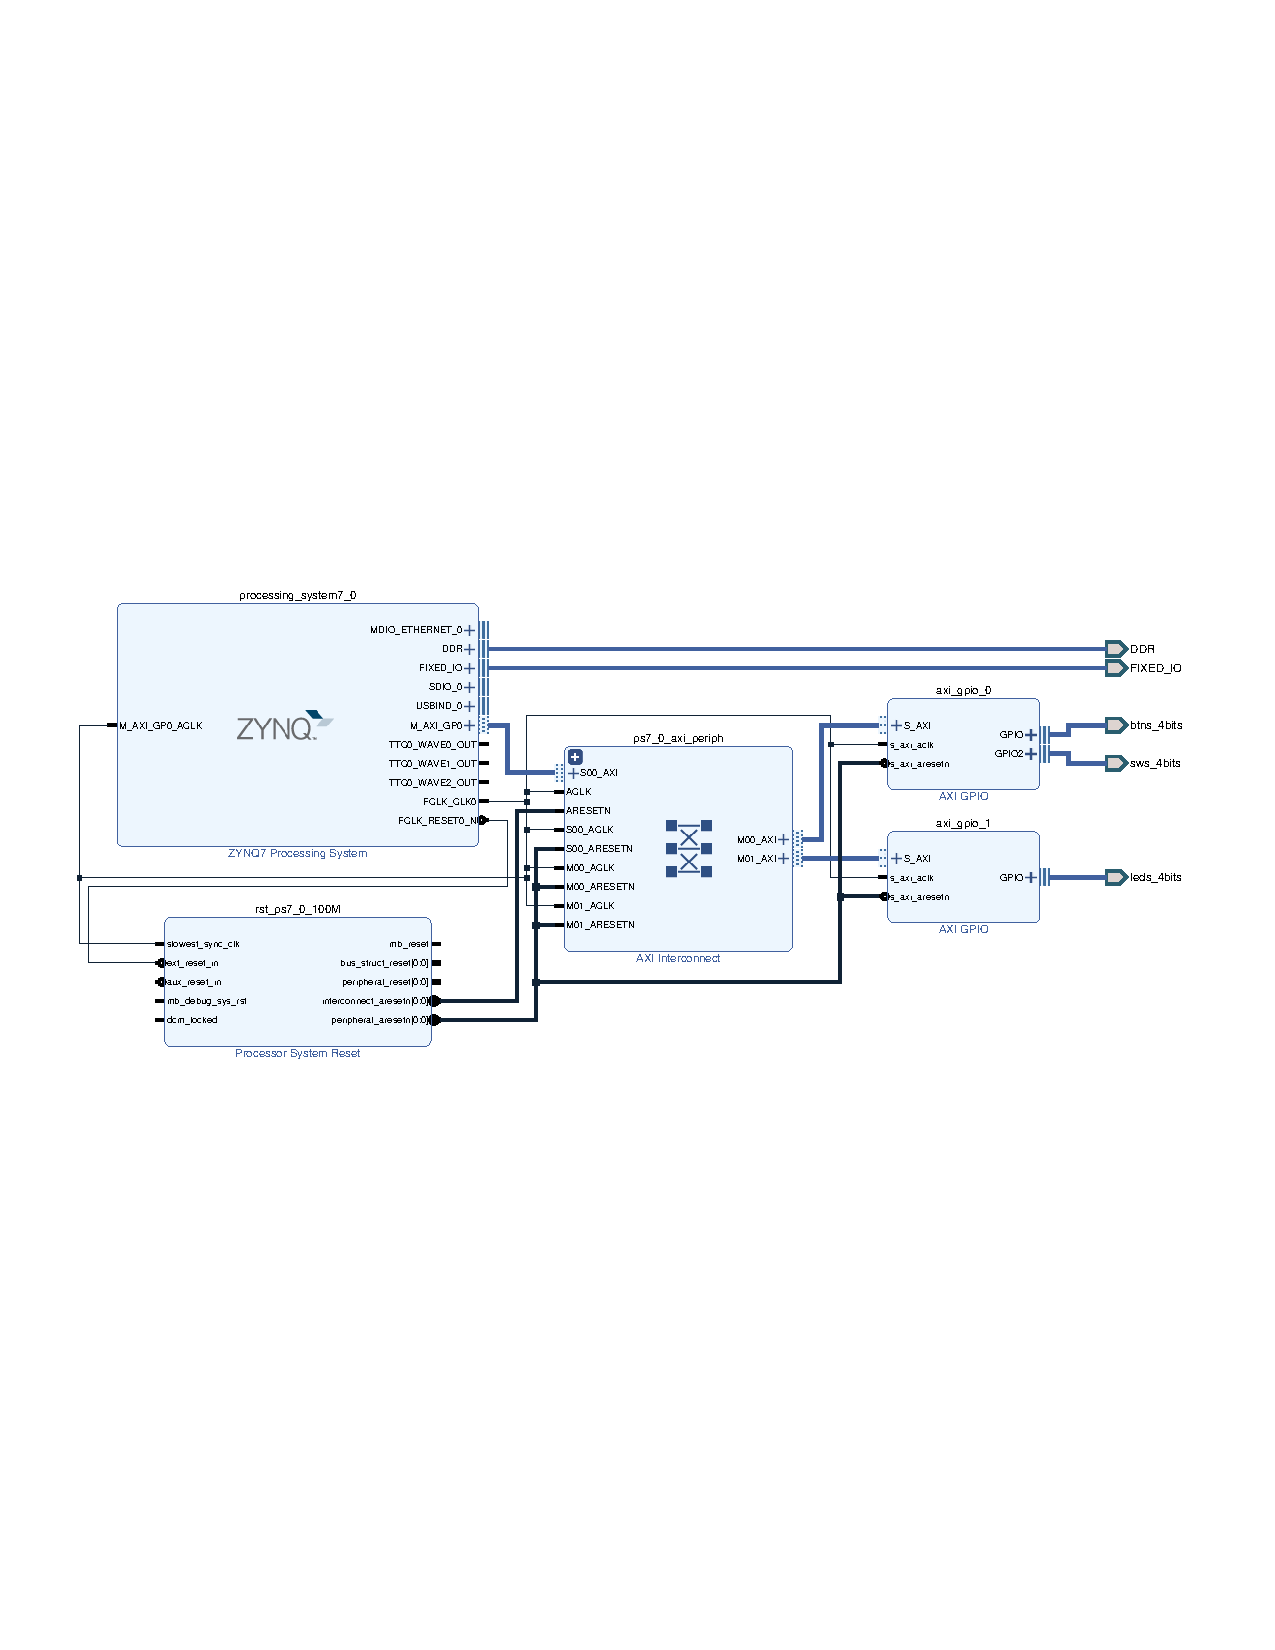
\includegraphics[trim = 10mm 100mm 10mm 100mm, width=0.9\linewidth]{./Bilder/Labor1_Aufgabe3_Bild1}
	\caption{LED Ansteuerung über AXI GPIO}
	\label{Labor1_Aufgabe3_Bild1}
\end{figure}
\FloatBarrier
\lstinputlisting[frame=single,caption=Lesen von Schaltern und Knöpfen,label=Labor1_Aufgabe3_Code1]{./Quellcode/Labor1_Aufgabe3_Code1.c}